\documentclass[mstat,12pt]{unswthesis}

\usepackage{color}
\usepackage{fancyvrb}
\newcommand{\VerbBar}{|}
\newcommand{\VERB}{\Verb[commandchars=\\\{\}]}
\DefineVerbatimEnvironment{Highlighting}{Verbatim}{commandchars=\\\{\}}
% Add ',fontsize=\small' for more characters per line
\usepackage{framed}
\definecolor{shadecolor}{RGB}{248,248,248}
\newenvironment{Shaded}{\begin{snugshade}}{\end{snugshade}}
\newcommand{\AlertTok}[1]{\textcolor[rgb]{0.94,0.16,0.16}{#1}}
\newcommand{\AnnotationTok}[1]{\textcolor[rgb]{0.56,0.35,0.01}{\textbf{\textit{#1}}}}
\newcommand{\AttributeTok}[1]{\textcolor[rgb]{0.13,0.29,0.53}{#1}}
\newcommand{\BaseNTok}[1]{\textcolor[rgb]{0.00,0.00,0.81}{#1}}
\newcommand{\BuiltInTok}[1]{#1}
\newcommand{\CharTok}[1]{\textcolor[rgb]{0.31,0.60,0.02}{#1}}
\newcommand{\CommentTok}[1]{\textcolor[rgb]{0.56,0.35,0.01}{\textit{#1}}}
\newcommand{\CommentVarTok}[1]{\textcolor[rgb]{0.56,0.35,0.01}{\textbf{\textit{#1}}}}
\newcommand{\ConstantTok}[1]{\textcolor[rgb]{0.56,0.35,0.01}{#1}}
\newcommand{\ControlFlowTok}[1]{\textcolor[rgb]{0.13,0.29,0.53}{\textbf{#1}}}
\newcommand{\DataTypeTok}[1]{\textcolor[rgb]{0.13,0.29,0.53}{#1}}
\newcommand{\DecValTok}[1]{\textcolor[rgb]{0.00,0.00,0.81}{#1}}
\newcommand{\DocumentationTok}[1]{\textcolor[rgb]{0.56,0.35,0.01}{\textbf{\textit{#1}}}}
\newcommand{\ErrorTok}[1]{\textcolor[rgb]{0.64,0.00,0.00}{\textbf{#1}}}
\newcommand{\ExtensionTok}[1]{#1}
\newcommand{\FloatTok}[1]{\textcolor[rgb]{0.00,0.00,0.81}{#1}}
\newcommand{\FunctionTok}[1]{\textcolor[rgb]{0.13,0.29,0.53}{\textbf{#1}}}
\newcommand{\ImportTok}[1]{#1}
\newcommand{\InformationTok}[1]{\textcolor[rgb]{0.56,0.35,0.01}{\textbf{\textit{#1}}}}
\newcommand{\KeywordTok}[1]{\textcolor[rgb]{0.13,0.29,0.53}{\textbf{#1}}}
\newcommand{\NormalTok}[1]{#1}
\newcommand{\OperatorTok}[1]{\textcolor[rgb]{0.81,0.36,0.00}{\textbf{#1}}}
\newcommand{\OtherTok}[1]{\textcolor[rgb]{0.56,0.35,0.01}{#1}}
\newcommand{\PreprocessorTok}[1]{\textcolor[rgb]{0.56,0.35,0.01}{\textit{#1}}}
\newcommand{\RegionMarkerTok}[1]{#1}
\newcommand{\SpecialCharTok}[1]{\textcolor[rgb]{0.81,0.36,0.00}{\textbf{#1}}}
\newcommand{\SpecialStringTok}[1]{\textcolor[rgb]{0.31,0.60,0.02}{#1}}
\newcommand{\StringTok}[1]{\textcolor[rgb]{0.31,0.60,0.02}{#1}}
\newcommand{\VariableTok}[1]{\textcolor[rgb]{0.00,0.00,0.00}{#1}}
\newcommand{\VerbatimStringTok}[1]{\textcolor[rgb]{0.31,0.60,0.02}{#1}}
\newcommand{\WarningTok}[1]{\textcolor[rgb]{0.56,0.35,0.01}{\textbf{\textit{#1}}}}


%%%%%%%%%%%%%%%%%%%%%%%%%%%%%%%%%%%%%%%%%%%%%%%%%%%%%%%%%%%%%%%%%%
% 
% OK...Now we get to some actual input.  The first part sets up
% the title etc that will appear on the front page
%
%%%%%%%%%%%%%%%%%%%%%%%%%%%%%%%%%%%%%%%%%%%%%%%%%%%%%%%%%%%%%%%%%

\title{Projet réalisé par\\[0.5cm] l'équipe Efficiency du groupe de TD2 \\[3cm]Rapport
de groupe des UE \newline  Bases de données + Sciences des Données 2}

\authornameonly{Hounsa Tylden, Oussaid El Amri Noha, Sylla
Mary-Yohana, Tall Aissatou }

\author{\Authornameonly}

\copyrightfalse
\figurespagefalse
\tablespagefalse

%%%%%%%%%%%%%%%%%%%%%%%%%%%%%%%%%%%%%%%%%%%%%%%%%%%%%%%%%%%%%%%%%
%
%  And now the document begins
%  The \beforepreface and \afterpreface commands puts the
%  contents page etc in
%
%%%%%%%%%%%%%%%%%%%%%%%%%%%%%%%%%%%%%%%%%%%%%%%%%%%%%%%%%%%%%%%%%%


%%%%%%%%%%%%%%%%%%%%%%%%%%%%%%%%%%%%%%%%%%%%%%%%%%%%%%%%%%%%%%%%%%%%%%%
%
%  A small sample UNSW Coursework Masters thesis file.
%  Any questions to Ian Doust i.doust@unsw.edu.au and/or Gery Geenens ggeenens@unsw.edu.au
%
%%%%%%%%%%%%%%%%%%%%%%%%%%%%%%%%%%%%%%%%%%%%%%%%%%%%%%%%%%%%%%%%%%%%%%%
%
%  The first part pulls in a UNSW Thesis class file.  This one is
%  slightly nonstandard and has been set up to do a couple of
%  things automatically
%
 
%%%%%%%%%%%%%%%%%
%% Precisely one of the next four lines should be uncommented.
%% Choose the one which matches your degree, uncomment it, and comment out the other two!
%\documentclass[mfin,12pt]{unswthesis}    %%  For Master of Financial Mathematics 
%\documentclass[mmath,12pt]{unswthesis}   %%  For Master of Mathematics
%\documentclass[mstat,12pt]{unswthesis}  %%  For Master of Statistics
%%%%%%%%%%%%%%%%%



\linespread{1}
%marge

\usepackage{amsfonts}
\usepackage{amssymb}
\usepackage{amsthm}
\usepackage{latexsym,amsmath}
\usepackage{graphicx}
\usepackage{afterpage}
\usepackage[colorlinks]{hyperref}
 \hypersetup{
     colorlinks=true,
     linkcolor=blue,
     filecolor=blue,
     citecolor= black,      
     urlcolor=cyan,
     }
\usepackage{textcomp}
\usepackage{longtable}
\usepackage{booktabs}
\usepackage{float}
\let\origfigure\figure
\let\endorigfigure\endfigure
\renewenvironment{figure}[1][2] {
    \expandafter\origfigure\expandafter[H]
} {
    \endorigfigure
}
\usepackage[T1]{fontenc}
\usepackage{ragged2e}
\def\tightlist{}
\usepackage[french]{babel}

%fonctionnement tableau
\usepackage{array}
\usepackage{calc}

%%%%%%%%%%%%%%%%%%%%%%%%%%%%%%%%%%%%%%%%%%%%%%%%%%%%%%%%%%%%%%%%%
%
%  The following are some simple LaTeX macros to give some
%  commonly used letters in funny fonts. You may need more or less of
%  these
%
\newcommand{\R}{\mathbb{R}}
\newcommand{\Q}{\mathbb{Q}}
\newcommand{\C}{\mathbb{C}}
\newcommand{\N}{\mathbb{N}}
\newcommand{\F}{\mathbb{F}}
\newcommand{\PP}{\mathbb{P}}
\newcommand{\T}{\mathbb{T}}
\newcommand{\Z}{\mathbb{Z}}
\newcommand{\B}{\mathfrak{B}}
\newcommand{\BB}{\mathcal{B}}
\newcommand{\M}{\mathfrak{M}}
\newcommand{\X}{\mathfrak{X}}
\newcommand{\Y}{\mathfrak{Y}}
\newcommand{\CC}{\mathcal{C}}
\newcommand{\E}{\mathbb{E}}
\newcommand{\cP}{\mathcal{P}}
\newcommand{\cS}{\mathcal{S}}
\newcommand{\A}{\mathcal{A}}
\newcommand{\ZZ}{\mathcal{Z}}
%%%%%%%%%%%%%%%%%%%%%%%%%%%%%%%%%%%%%%%%%%%%%%%%%%%%%%%%%%%%%%%%%%%%%
%
% The following are much more esoteric commands that I have left in
% so that this file still processes. Use or delete as you see fit
%
\newcommand{\bv}[1]{\mbox{BV($#1$)}}
\newcommand{\comb}[2]{\left(\!\!\!\begin{array}{c}#1\\#2\end{array}\!\!\!\right)
}
\newcommand{\Lat}{{\rm Lat}}
\newcommand{\var}{\mathop{\rm var}}
\newcommand{\Pt}{{\mathcal P}}
\def\tr(#1){{\rm trace}(#1)}
\def\Exp(#1){{\mathbb E}(#1)}
\def\Exps(#1){{\mathbb E}\sparen(#1)}
\newcommand{\floor}[1]{\left\lfloor #1 \right\rfloor}
\newcommand{\ceil}[1]{\left\lceil #1 \right\rceil}
\newcommand{\hatt}[1]{\widehat #1}
\newcommand{\modeq}[3]{#1 \equiv #2 \,(\text{mod}\, #3)}
\newcommand{\rmod}{\,\mathrm{mod}\,}
\newcommand{\p}{\hphantom{+}}
\newcommand{\vect}[1]{\mbox{\boldmath $ #1 $}}
\newcommand{\reff}[2]{\ref{#1}.\ref{#2}}
\newcommand{\psum}[2]{\sum_{#1}^{#2}\!\!\!'\,\,}
\newcommand{\bin}[2]{\left( \begin{array}{@{}c@{}}
				#1 \\ #2
			\end{array}\right)	}
%
%  Macros - some of these are in plain TeX (gasp!)
%
\newcommand{\be}{($\beta$)}
\newcommand{\eqp}{\mathrel{{=}_p}}
\newcommand{\ltp}{\mathrel{{\prec}_p}}
\newcommand{\lep}{\mathrel{{\preceq}_p}}
\def\brack#1{\left \{ #1 \right \}}
\def\bul{$\bullet$\ }
\def\cl{{\rm cl}}
\let\del=\partial
\def\enditem{\par\smallskip\noindent}
\def\implies{\Rightarrow}
\def\inpr#1,#2{\t \hbox{\langle #1 , #2 \rangle} \t}
\def\ip<#1,#2>{\langle #1,#2 \rangle}
\def\lp{\ell^p}
\def\maxb#1{\max \brack{#1}}
\def\minb#1{\min \brack{#1}}
\def\mod#1{\left \vert #1 \right \vert}
\def\norm#1{\left \Vert #1 \right \Vert}
\def\paren(#1){\left( #1 \right)}
\def\qed{\hfill \hbox{$\Box$} \smallskip}
\def\sbrack#1{\Bigl \{ #1 \Bigr \} }
\def\ssbrack#1{ \{ #1 \} }
\def\smod#1{\Bigl \vert #1 \Bigr \vert}
\def\smmod#1{\bigl \vert #1 \bigr \vert}
\def\ssmod#1{\vert #1 \vert}
\def\sspmod#1{\vert\, #1 \, \vert}
\def\snorm#1{\Bigl \Vert #1 \Bigr \Vert}
\def\ssnorm#1{\Vert #1 \Vert}
\def\sparen(#1){\Bigl ( #1 \Bigr )}

\newcommand\blankpage{%
    \null
    \thispagestyle{empty}%
    \addtocounter{page}{-1}%
    \newpage}

%%%%%%%%%%%%%%%%%%%%%%%%%%%%%%%
%
% These environments allow you to get nice numbered headings
%  for your Theorems, Definitions etc.  
%
%  Environments
%
%%%%%%%%%%%%%%%%%%%%%%%%%%%%%%%

\newtheorem{theorem}{Theorem}[section]
\newtheorem{lemma}[theorem]{Lemma}
\newtheorem{proposition}[theorem]{Proposition}
\newtheorem{corollary}[theorem]{Corollary}
\newtheorem{conjecture}[theorem]{Conjecture}
\newtheorem{definition}[theorem]{Definition}
\newtheorem{example}[theorem]{Example}
\newtheorem{remark}[theorem]{Remark}
\newtheorem{question}[theorem]{Question}
\newtheorem{notation}[theorem]{Notation}
\numberwithin{equation}{section}

%%%%%%%%%%%%%%%%%%%%%%%%%%%%%%%%%%%%%%%%%%%%%%%%%%%%%%%%%%%%%%%%%%
%
%  If you've got some funny special words that LaTeX might not
% hyphenate properly, you can give it a helping hand:
%

\hyphenation{Mar-cin-kie-wicz Rade-macher}


\newlength{\cslhangindent}
\setlength{\cslhangindent}{1.5em}
\newlength{\csllabelwidth}
\setlength{\csllabelwidth}{3em}
\newenvironment{CSLReferences}[2] % #1 hanging-ident, #2 entry spacing
 {% don't indent paragraphs
  \setlength{\parindent}{0pt}
  % turn on hanging indent if param 1 is 1
  \ifodd #1 \everypar{\setlength{\hangindent}{\cslhangindent}}\ignorespaces\fi
  % set entry spacing
  \ifnum #2 > 0
  \setlength{\parskip}{#2\baselineskip}
  \fi
 }%
 {}
\usepackage{calc} % for \widthof, \maxof
\newcommand{\CSLBlock}[1]{#1\hfill\break}
\newcommand{\CSLLeftMargin}[1]{\parbox[t]{\maxof{\widthof{#1}}{\csllabelwidth}}{#1}}
\newcommand{\CSLRightInline}[1]{\parbox[t]{\linewidth}{#1}}
\newcommand{\CSLIndent}[1]{\hspace{\cslhangindent}#1}






\renewcommand{\contentsname}{Table des matières}

\renewcommand{\chaptername}{Chapitre}




\begin{document}

\beforepreface

%\afterpage{\blankpage}

% plagiarism

\prefacesection{Déclaration de non plagiat}

\vskip 2pc \noindent Nous déclarons que ce rapport est le fruit de notre seul travail, à part lorsque cela est indiqué  explicitement. 

\vskip 2pc  \noindent Nous acceptons que la personne évaluant ce rapport puisse, pour les besoins de cette évaluation:
\begin{itemize}
\item la reproduire et en fournir une copie à un autre membre de l'université; et/ou,
\item en communiquer une copie à un service en ligne de détection de plagiat (qui pourra en retenir une copie pour les besoins d'évaluation future).
\end{itemize}

\vskip 2pc \noindent Nous certifions que nous avons lu et compris les règles ci-dessus.

\vskip 2pc \noindent En signant cette déclaration, nous acceptons ce qui précède.
\vskip 2pc \noindent
%%Signature: \rule{7cm}{0.25pt} \hfill Date: \rule{4cm}{0.25pt} \\[1cm]
%%Signature: \rule{7cm}{0.25pt} \hfill Date: \rule{4cm}{0.25pt} \\[1cm]
%%Signature: \rule{7cm}{0.25pt} \hfill Date: \rule{4cm}{0.25pt} \\[1cm]
%%Signature: \rule{7cm}{0.25pt} \hfill Date: \rule{4cm}{0.25pt} \\[1cm]
%%\vskip 1pc
Signature : Hounsa Tylden \hfill Date: 01/04/2026\\[1cm]
Signature : Oussaid El Amri Noha \hfill Date: 01/04/2026 \\[1cm]
Signature : Sylla Mary-Yohana \hfill Date: 01/04/2026 \\[1cm]
Signature : Tall Aissatou \hfill Date: 01/04/2026 \\[1cm]


%\textcolor{red}{Mettre à jour la date.}

{\bigskip\bigskip\bigskip\noindent} \today
%\afterpage{\blankpage}

% Acknowledgements are optional


\prefacesection{Remerciements}

{\bigskip}Nos plus sincères remerciements vont à notre encadrant
pédagogique pour les conseils avisés sur notre travail.\\[1cm] Nous
remercions également Kaggle et l'Organisation Mondiale de la Santé pour
la mise à disposition publique des jeux de données utilisés dans ce
projet.\\[1cm] 

{\bigskip\bigskip\bigskip\noindent} \today

%\afterpage{\blankpage}

% Abstract

\prefacesection{Résumé}

La pollution atmosphérique constitue l'une des principales causes de
mortalité évitable à l'échelle mondiale. Ce rapport croise des données
environnementales issues de Kaggle (23 464 villes, indice AQI et
concentration en PM2.5) avec des statistiques sanitaires de l'OMS (taux
de mortalité par maladies liées à la pollution, 183 pays, année 2016),
afin d'examiner la corrélation entre qualité de l'air urbaine et
mortalité nationale. Après constitution d'une base de données
relationnelle sous MySQL (tables PAYS, VILLE et SANTE), une démarche en
trois étapes révèle l'importance du choix de l'indicateur de mortalité :
l'absence de corrélation sur les taux bruts (r = 0,035) s'explique par
un biais démographique, corrigé par l'utilisation des taux standardisés
selon l'âge fournis par l'OMS. Après identification et exclusion d'une
valeur aberrante, une corrélation positive modérée et statistiquement
significative est établie entre le niveau moyen de PM2.5 par pays et le
taux de mortalité standardisé (r = 0,28, p \textless{} 0,001). Un modèle
de régression linéaire simple quantifie cet effet, et une segmentation
par K-means identifie trois profils de pays distincts. Ces résultats
soulignent l'importance du choix des indicateurs dans ce type d'étude et
plaident pour le développement de données de morbidité comparables à
l'échelle internationale.

%\afterpage{\blankpage}


\afterpreface





%%%%%%%%%%%%%%%%%%%%%%%%%%%%%%%%%%%%%%%%%%%%%%%%%%%%%%%%%%%%%%%%%%
%
% Now we can start on the first chapter
% Within chapters we have sections, subsections and so forth
%
%%%%%%%%%%%%%%%%%%%%%%%%%%%%%%%%%%%%%%%%%%%%%%%%%%%%%%%%%%%%%%%%%%



%%%%%%%%%%%%%%%%%%%%%%%%%%%%%%%%%%%%%

%\afterpage{\blankpage}


\chapter{Introduction}\label{introduction}

\section{Présentation du contexte et
problématique}\label{pruxe9sentation-du-contexte-et-probluxe9matique}

La dégradation de la qualité de l'air est aujourd'hui reconnue comme
l'une des menaces les plus graves pour la santé publique mondiale. Selon
les rapports de l'Organisation Mondiale de la Santé (OMS), l'exposition
prolongée aux polluants atmosphériques, et plus particulièrement aux
particules fines (PM2.5), est directement associée à l'augmentation des
pathologies respiratoires chroniques et des décès prématurés. Les
particules PM2, dont le diamètre aérodynamique est inférieur à 2,5
micromètres, sont particulièrement dangereuses car elles pénètrent
profondément dans les alvéoles pulmonaires et peuvent atteindre la
circulation sanguine, provoquant des effets systémiques bien au-delà du
seul appareil respiratoire.

L'enjeu de ce projet est de croiser des mesures environnementales
urbaines avec des indicateurs de mortalité pour vérifier la réalité de
cet impact à l'échelle globale. Notre recherche s'articule autour de la
question suivante :

\bigskip

\begin{center}
\textbf{Existe-t-il une corrélation significative entre les niveaux de pollution urbaine (AQI et PM2.5) et les taux de mortalité par maladies respiratoires à l'échelle mondiale ?}
\end{center}
\medskip
\justifying

Cette question est cruciale car elle permet d'évaluer l'efficacité des
politiques environnementales actuelles. Si une corrélation forte est
établie, cela justifierait des mesures plus restrictives sur les
émissions polluantes dans les zones urbaines denses, afin de réduire la
pression sur les systèmes de santé publique. Les résultats de cette
étude pourront également servir d'appui scientifique à des organisations
souhaitant prioriser leurs interventions géographiques.

\section{Responsabilités et composition de
l'équipe}\label{responsabilituxe9s-et-composition-de-luxe9quipe}

\medskip

\begin{itemize}
\tightlist
\item
  \textbf{Tylden Hounsa} : Étudiant n\textsuperscript{o}22412555,
  Responsable du rapport et des analyses SQL (Rédacteur principal du
  .Rmd).
\end{itemize}

\medskip

\begin{itemize}
\tightlist
\item
  \textbf{Noha Oussaid El Amri} : Étudiante
  n\textsuperscript{o}22413984, Responsable de la collecte et du
  nettoyage des données (\textit{Data Cleaning}).
\end{itemize}

\medskip

\begin{itemize}
\tightlist
\item
  \textbf{Mary-Yohana Sylla} : Étudiante n\textsuperscript{o}22414031,
  Responsable de la modélisation de la base de données (MCD/MOD).
\end{itemize}

\medskip

\begin{itemize}
\tightlist
\item
  \textbf{Aissatou Tall} : Étudiante n\textsuperscript{o}22414034,
  Responsable des visualisations graphiques et de l'analyse
  exploratoire.
\end{itemize}

\section{Quelques détails
techniques}\label{quelques-duxe9tails-techniques}

Pour la réalisation de ce rapport, nous utilisons \textbf{R Markdown}
via \textbf{RStudio}, ce qui permet d'intégrer directement nos scripts
d'analyse au sein du document et d'en assurer la reproductibilité. La
qualité rédactionnelle est vérifiée via l'outil LanguageTool
(\url{https://languagetool.org/fr}). Les schémas relationnels sont
conçus avec \textbf{Mocodo} (\url{https://www.mocodo.net/}) pour le MCD,
et avec le designer de \textbf{PHPMyAdmin} pour le MOD.

\chapter{Base de données}\label{base-de-donnuxe9es}

\section{Provenance des données}\label{provenance-des-donnuxe9es}

Nous avons sélectionné deux jeux de données provenant de sources
officielles et distinctes pour répondre à notre problématique :

\bigskip

\textbf{Données de Pollution (Source Environnementale) :}

\begin{itemize}
  \item Lien : \href{https://www.kaggle.com/datasets/hasibalmuzdadid/global-air-pollution-dataset/data}{Kaggle -- Global Air Pollution Dataset (basé sur OpenAQ)}.
  \item Description : Ce fichier recense les indices de qualité de l'air (AQI) et les concentrations de plusieurs polluants pour plus de 23\,000 villes à travers le monde. Nous l'avons retenu pour sa granularité urbaine et son étendue géographique internationale.
  \item Format : .csv $|$ Taille : 1\,593 ko $|$ Dimensions : 23\,464 lignes $\times$ 12 colonnes.
\end{itemize}

\bigskip

\textbf{Données de Santé (Source Médicale) :}

\begin{itemize}
  \item Lien : \href{https://www.kaggle.com/datasets/utkarshxy/who-worldhealth-statistics-2020-complete?select=airPollutionDeathRate.csv}{OMS -- Air Pollution Death Rate}.
  \item Description : Statistiques de mortalité attribuable à la pollution atmosphérique, publiées par l'OMS pour l'année 2016 et couvrant 183 pays. Nous avons filtré les données pour ne conserver que les indicateurs relatifs aux maladies respiratoires et cardiovasculaires directement liées à la pollution.
  \item Format : .csv $|$ Taille : 1\,036 ko $|$ Dimensions : 6\,589 lignes $\times$ 6 colonnes.
\end{itemize}

\bigskip

\textbf{Population étudiée :} L'unité statistique retenue est le
\textbf{pays}. Bien que les données de pollution soient mesurées à
l'échelle de la ville, nous les agrégeons par pays, via une moyenne du
PM2.5, pour permettre la jointure avec les données de l'OMS, disponibles
uniquement à l'échelle nationale. Cette agrégation introduit cepensant
une perte de granularité explicitée dans la partie Discussion.

\section{Descriptif des tables}\label{descriptif-des-tables}

Après nettoyage et structuration des données, nous avons constitué trois
tables : PAYS, VILLE et SANTE. Leurs caractéristiques sont détaillées
ci-dessous.

\medskip

\begin{table}[H]
\centering
\renewcommand{\arraystretch}{1.3}
\begin{tabular}{|p{3cm}|p{3.5cm}|p{3cm}|p{3cm}|}
\hline
\textbf{Nom colonne} & \textbf{Type} & \textbf{Signification} & \textbf{Caractéristique} \\ \hline
id\_pays & INT NOT NULL & Identifiant numérique unique & Clé primaire, séquentiel 1--192 \\ \hline
nom\_pays & VARCHAR(100) NOT NULL & Nom du pays (en anglais) & 192 valeurs uniques \\ \hline
\end{tabular}
\medskip
\caption{Table PAYS (2 colonnes $\times$ 192 lignes)}
\end{table}
\begin{table}[H]
\centering
\renewcommand{\arraystretch}{1.3}
\begin{tabular}{|p{3cm}|p{3.5cm}|p{3cm}|p{4.5cm}|}
\hline
\textbf{Nom colonne} & \textbf{Type} & \textbf{Signification} & \textbf{Caractéristique} \\ \hline
id\_stat & INT NOT NULL & Identifiant de la ligne & Clé primaire \\ \hline
indicateur & VARCHAR(25) & Type de taux de mortalité & \texttt{attributable}, \texttt{attributable\_age\_std} \\ \hline
maladie & VARCHAR(150) & Cause de décès & Total, Lower respiratory infections, Trachea bronchus lung cancers, Ischaemic heart disease, Stroke, Chronic obstructive pulmonary disease \\ \hline
valeur\_taux & FLOAT & Taux de mortalité pour 100\,000 hab. & 1,00 -- 99,91 \\ \hline
periode & INT & Année de relevé & 2016 \\ \hline
sexe & VARCHAR(20) & Sexe concerné & Female, Male, Both sexes \\ \hline
id\_pays & INT NOT NULL & Référence au pays & Clé étrangère $\rightarrow$ PAYS \\ \hline
\end{tabular}
\medskip
\caption{Table SANTE (7 colonnes $\times$ 6\,588 lignes)}
\end{table}
\begin{table}[H]
\centering
\renewcommand{\arraystretch}{1.3}
\begin{tabular}{|p{3cm}|p{3.5cm}|p{3cm}|p{4.5cm}|}
\hline
\textbf{Nom colonne} & \textbf{Type} & \textbf{Signification} & \textbf{Caractéristique} \\ \hline
id\_ville & INT NOT NULL & Identifiant de la ville & Clé primaire \\ \hline
nom\_ville & VARCHAR(150) NOT NULL & Nom de la ville & $\approx$23\,000 villes distinctes \\ \hline
aqi\_value & INT & Indice de Qualité de l'Air & 6 -- 500 \\ \hline
pm25\_value & INT & Concentration en PM2.5 ($\mu$g/m$^3$) & 0 -- 500 \\ \hline
aqi\_category & VARCHAR(50) & Catégorie de qualité de l'air & Good, Moderate, Unhealthy\_for\_Sensitive\_Groups, Unhealthy, Very\_Unhealthy, Hazardous \\ \hline
id\_pays & INT NOT NULL & Référence au pays & Clé étrangère $\rightarrow$ PAYS \\ \hline
\end{tabular}
\medskip
\caption{Table VILLE (6 colonnes $\times$ 23\,035 lignes)}
\end{table}

\section{Modèles MCD et MOD}\label{moduxe8les-mcd-et-mod}

Le Modèle Conceptuel de Données (MCD) a été réalisé avec Mocodo. Il
représente les trois entités PAYS, VILLE et SANTE, reliées par des
associations de cardinalités (1,n) : un pays peut être associé à
plusieurs villes et à plusieurs entrées sanitaires.

\begin{figure}
\centering
{MCD réalisé avec Mocodo.}
\caption{MCD réalisé avec Mocodo.}\label{mcd}
\end{figure}

\bigskip

Le Modèle Organisationnel de Données (MOD) a été généré via le designer
de PHPMyAdmin. Il formalise les types de données et les contraintes de
clés étrangères entre les tables.

\begin{figure}
\centering
{MOD généré via le designer de PHPMyAdmin.}
\caption{MOD généré via le designer de PHPMyAdmin.}\label{mod}
\end{figure}

\section{Import des données}\label{import-des-donnuxe9es}

Afin de garantir l'intégrité référentielle et la qualité des analyses
futures, un processus rigoureux de nettoyage et de structuration a été
mené à l'aide du logiciel \textbf{LibreOffice Calc}. Ce traitement a
permis de passer de deux fichiers CSV « plats » à une structure
relationnelle conforme à notre MCD.

\subsection{Création de la table de référence :
PAYS}\label{cruxe9ation-de-la-table-de-ruxe9fuxe9rence-pays}

La table \texttt{PAYS} sert de pivot central entre les deux sources de
données. Son élaboration a suivi les étapes suivantes :

\medskip

\begin{itemize}
  \item \textbf{Extraction et fusion :} Les colonnes \texttt{Country} (base pollution) et \texttt{Location} (base santé) ont été consolidées dans une feuille unique afin d'obtenir la liste complète des pays présents dans les deux sources.
  \item \textbf{Dédoublonnage :} La fonction native \textbf{``Supprimer les doublons''} a permis d'obtenir une liste de nations uniques. Les noms étant uniformément en anglais dans les deux sources, aucune erreur de traduction n'a été relevée. Quelques doublons mineurs (ex.\ : « Côte d'Ivoire » présent deux fois sous des encodages différents) ont été corrigés manuellement.
  \item \textbf{Indexation :} Les pays ont été triés par ordre alphabétique, puis un identifiant unique a été attribué. La colonne a été renommée \texttt{id\_pays} et constitue la clé primaire de la table.
\end{itemize}

\subsection{Structuration de la table
VILLE}\label{structuration-de-la-table-ville}

Pour la table \texttt{VILLE}, une sélection et un enrichissement des
données ont été opérés :

\medskip

\begin{itemize}
  \item \textbf{Sélection d'attributs :} Parmi les 12 colonnes du fichier source, seules 4 ont été conservées et renommées : \texttt{nom\_ville}, \texttt{aqi\_value}, \texttt{pm25\_value} et \texttt{aqi\_category}. Les colonnes relatives aux autres polluants (NO2, CO, O3) ont été écartées, car notre problématique se concentre sur les PM2.5.
  \item \textbf{Jointure logique :} La fonction \textbf{\texttt{RECHERCHEV}} a permis d'attribuer à chaque ville son identifiant \texttt{id\_pays} en recherchant le nom du pays associé dans la table \texttt{PAYS}.
  \item \textbf{Nettoyage :} La colonne textuelle \texttt{Country} a ensuite été supprimée. Les lignes présentant des données manquantes ou des villes sans correspondance nationale ont été éliminées pour ne pas biaiser les traitements statistiques.
\end{itemize}

\subsection{Structuration de la table
SANTE}\label{structuration-de-la-table-sante}

Le traitement de la base de l'OMS a nécessité un filtrage et un
remapping des champs :

\medskip

\begin{itemize}
  \item \textbf{Mapping des champs :} Les colonnes \texttt{Indicator}, \texttt{Dim2}, \texttt{Period} et \texttt{Dim1} ont été renommées respectivement en \texttt{indicateur}, \texttt{maladie}, \texttt{periode} et \texttt{sexe}. Les intitulés verbeux de la colonne \texttt{indicateur} ont été simplifiés : « Ambient and household air pollution attributable death rate (per 100 000 population) » devient \texttt{attributable}, et sa variante standardisée par l'âge devient \texttt{attributable\_age\_std}.
  \item \textbf{Référencement :} Comme pour les villes, la fonction \textbf{\texttt{RECHERCHEV}} a permis de substituer le nom du pays par son identifiant numérique \texttt{id\_pays}, garantissant la cohérence des futures jointures SQL.
\end{itemize}

\subsection{Importation sous
PHPMyAdmin}\label{importation-sous-phpmyadmin}

Une fois les trois fichiers préparés au format \textbf{CSV (UTF-8)}, le
déploiement dans MySQL s'est déroulé en deux temps :

\medskip

\begin{itemize}
  \item \textbf{Script de structure :} Exécution d'un fichier \texttt{.sql} définissant les tables, les types de données et les contraintes d'intégrité. Le code utilisé est forni en pièce jointe au document.
\end{itemize}

\medskip

\medskip

\begin{itemize}
  \item \textbf{Peuplement :} Importation successive des fichiers \texttt{pays.csv}, \texttt{ville.csv} et \texttt{sante.csv} via l'interface d'import de PHPMyAdmin. L'ordre d'importation a été scrupuleusement respecté, la table parente \texttt{PAYS} en premier, pour éviter toute violation de contrainte d'intégrité référentielle.
\end{itemize}

\section{Requêtes réalisées}\label{requuxeates-ruxe9alisuxe9es}

Les requêtes suivantes constituent le cœur de notre analyse SQL. Elles
ont été conçues pour répondre progressivement à notre problématique, en
allant du simple descriptif à la mise en relation entre pollution et
mortalité. Pour chacune, nous présentons la question posée en langage
naturel, la requête SQL, puis le résultat obtenu et son interprétation.

\medskip

\subsection{Requête 1 : Quels sont les dix pays présentant la plus forte
concentration moyenne en PM2.5
?}\label{requuxeate-1-quels-sont-les-dix-pays-pruxe9sentant-la-plus-forte-concentration-moyenne-en-pm2.5}

\textbf{En langage naturel :} On cherche à identifier les pays les plus
exposés aux particules fines en agrégeant, pour chaque pays, la moyenne
des concentrations PM2.5 relevées dans ses villes. Le résultat est trié
par ordre décroissant et limité aux dix premiers.

\begin{Shaded}
\begin{Highlighting}[]
\KeywordTok{SELECT}\NormalTok{ P.nom\_pays,}
       \FunctionTok{ROUND}\NormalTok{(}\FunctionTok{AVG}\NormalTok{(V.pm25\_value), }\DecValTok{1}\NormalTok{) }\KeywordTok{AS}\NormalTok{ pm25\_moyen,}
       \FunctionTok{COUNT}\NormalTok{(V.id\_ville)           }\KeywordTok{AS}\NormalTok{ nb\_villes}
\KeywordTok{FROM}\NormalTok{ PAYS  P}
\KeywordTok{JOIN}\NormalTok{ VILLE V }\KeywordTok{ON}\NormalTok{ P.id\_pays }\OperatorTok{=}\NormalTok{ V.id\_pays}
\KeywordTok{GROUP} \KeywordTok{BY}\NormalTok{ P.nom\_pays}
\KeywordTok{ORDER} \KeywordTok{BY}\NormalTok{ pm25\_moyen }\KeywordTok{DESC}
\KeywordTok{LIMIT} \DecValTok{10}\NormalTok{;}
\end{Highlighting}
\end{Shaded}

\begin{longtable}[]{@{}lrr@{}}
\caption{Displaying records 1 - 10}\tabularnewline
\toprule\noalign{}
nom\_pays & pm25\_moyen & nb\_villes \\
\midrule\noalign{}
\endfirsthead
\toprule\noalign{}
nom\_pays & pm25\_moyen & nb\_villes \\
\midrule\noalign{}
\endhead
\bottomrule\noalign{}
\endlastfoot
Republic of Korea & 415.0 & 1 \\
Bahrain & 188.0 & 1 \\
Mauritania & 179.0 & 4 \\
Pakistan & 173.1 & 307 \\
Aruba & 163.0 & 1 \\
Kuwait & 162.0 & 3 \\
United Arab Emirates & 152.7 & 3 \\
Senegal & 152.4 & 33 \\
India & 149.5 & 2488 \\
Saudi Arabia & 149.3 & 14 \\
\end{longtable}

\textbf{Interprétation :} Les pays en tête de ce classement sont
majoritairement situés en Asie du Sud et en Afrique subsaharienne. Ces
résultats reflètent des facteurs structurels : forte densité
industrielle non régulée, combustion de biomasse pour la cuisson
domestique, et insuffisance des politiques environnementales. À titre de
référence, la valeur guide de l'OMS pour le PM2.5 annuel est fixée à 5
µg/m³, un seuil largement dépassé par l'ensemble de ces pays.

\medskip

\subsection{Requête 2 : Quels pays présentent un AQI moyen supérieur à
la moyenne mondiale
?}\label{requuxeate-2-quels-pays-pruxe9sentent-un-aqi-moyen-supuxe9rieur-uxe0-la-moyenne-mondiale}

\textbf{En langage naturel :} On calcule d'abord la moyenne mondiale de
l'AQI via une sous-requête, puis on sélectionne les pays dont la moyenne
nationale dépasse ce seuil. Cette approche utilise la clause
\texttt{HAVING} combinée à une sous-requête imbriquée.

\begin{Shaded}
\begin{Highlighting}[]
\KeywordTok{SELECT}\NormalTok{ P.nom\_pays,}
       \FunctionTok{ROUND}\NormalTok{(}\FunctionTok{AVG}\NormalTok{(V.aqi\_value), }\DecValTok{1}\NormalTok{) }\KeywordTok{AS}\NormalTok{ aqi\_moyen}
\KeywordTok{FROM}\NormalTok{ PAYS  P}
\KeywordTok{JOIN}\NormalTok{ VILLE V }\KeywordTok{ON}\NormalTok{ P.id\_pays }\OperatorTok{=}\NormalTok{ V.id\_pays}
\KeywordTok{GROUP} \KeywordTok{BY}\NormalTok{ P.nom\_pays}
\KeywordTok{HAVING}\NormalTok{ aqi\_moyen }\OperatorTok{\textgreater{}}\NormalTok{ (}
           \KeywordTok{SELECT} \FunctionTok{AVG}\NormalTok{(aqi\_value)}
           \KeywordTok{FROM}\NormalTok{ VILLE}
\NormalTok{         )}
\KeywordTok{ORDER} \KeywordTok{BY}\NormalTok{ aqi\_moyen }\KeywordTok{DESC}\NormalTok{;}
\end{Highlighting}
\end{Shaded}

\begin{longtable}[]{@{}lr@{}}
\caption{Displaying records 1 - 10}\tabularnewline
\toprule\noalign{}
nom\_pays & aqi\_moyen \\
\midrule\noalign{}
\endfirsthead
\toprule\noalign{}
nom\_pays & aqi\_moyen \\
\midrule\noalign{}
\endhead
\bottomrule\noalign{}
\endlastfoot
Republic of Korea & 421.0 \\
Bahrain & 188.0 \\
Mauritania & 179.0 \\
Pakistan & 178.8 \\
United Arab Emirates & 163.7 \\
Aruba & 163.0 \\
Kuwait & 162.0 \\
Qatar & 157.5 \\
India & 153.0 \\
Senegal & 152.4 \\
\end{longtable}

\textbf{Interprétation :} La sous-requête imbriquée
(\texttt{HAVING\ ...\ \textgreater{}\ SELECT\ AVG(...)}) est une
technique SQL avancée permettant de filtrer dynamiquement sans avoir à
coder en dur le seuil. On dénombre une cinquantaine de pays dont l'AQI
moyen dépasse la valeur mondiale. Ce résultat met en évidence une
inégalité géographique marquée : les pays à faible revenu concentrent la
quasi-totalité des situations à risque.

\medskip

\subsection{Requête 3 : Comment la mortalité évolue-t-elle selon la
catégorie d'AQI
?}\label{requuxeate-3-comment-la-mortalituxe9-uxe9volue-t-elle-selon-la-catuxe9gorie-daqi}

\textbf{En langage naturel :} On commence notre croisement de données en
comparant les catégories qualitatives d'AQI avec la mortalité
respiratoire moyenne. Pour éviter les doublons statistiques, on isole
les données Both sexes et l'indicateur attributable. Le classement est
fait par ordre croissant d'AQI (du moins pollué au plus pollué).

\begin{Shaded}
\begin{Highlighting}[]
\KeywordTok{SELECT}\NormalTok{ V.aqi\_category, }
       \FunctionTok{ROUND}\NormalTok{(}\FunctionTok{AVG}\NormalTok{(V.aqi\_value), }\DecValTok{1}\NormalTok{) }\KeywordTok{AS}\NormalTok{ aqi\_moyen, }
       \FunctionTok{ROUND}\NormalTok{(}\FunctionTok{AVG}\NormalTok{(S.valeur\_taux), }\DecValTok{2}\NormalTok{) }\KeywordTok{AS}\NormalTok{ mortalite\_moyenne }
\KeywordTok{FROM}\NormalTok{ VILLE V }
\KeywordTok{JOIN}\NormalTok{ PAYS P }\KeywordTok{ON}\NormalTok{ V.id\_pays }\OperatorTok{=}\NormalTok{ P.id\_pays }
\KeywordTok{JOIN}\NormalTok{ SANTE S }\KeywordTok{ON}\NormalTok{ P.id\_pays }\OperatorTok{=}\NormalTok{ S.id\_pays }
\KeywordTok{WHERE}\NormalTok{ S.maladie }\OperatorTok{=} \StringTok{\textquotesingle{}Lower respiratory infections\textquotesingle{}} 
  \KeywordTok{AND}\NormalTok{ S.sexe }\OperatorTok{=} \StringTok{\textquotesingle{}Both sexes\textquotesingle{}}
  \KeywordTok{AND}\NormalTok{ S.}\KeywordTok{indicator} \OperatorTok{=} \StringTok{\textquotesingle{}attributable\textquotesingle{}}
\KeywordTok{GROUP} \KeywordTok{BY}\NormalTok{ V.aqi\_category }
\KeywordTok{ORDER} \KeywordTok{BY}\NormalTok{ aqi\_moyen }\KeywordTok{ASC}\NormalTok{;}
\end{Highlighting}
\end{Shaded}

\begin{longtable}[]{@{}lrr@{}}
\caption{6 records}\tabularnewline
\toprule\noalign{}
aqi\_category & aqi\_moyen & mortalite\_moyenne \\
\midrule\noalign{}
\endfirsthead
\toprule\noalign{}
aqi\_category & aqi\_moyen & mortalite\_moyenne \\
\midrule\noalign{}
\endhead
\bottomrule\noalign{}
\endlastfoot
Good & 36.5 & 8.47 \\
Moderate & 66.5 & 11.67 \\
Unhealthy\_for\_Sensitive\_Groups & 121.2 & 18.76 \\
Unhealthy & 166.7 & 23.24 \\
Very\_Unhealthy & 228.2 & 22.74 \\
Hazardous & 440.9 & 28.25 \\
\end{longtable}

\textbf{Interprétation :} En observant les résultats, on constate que la
mortalité respiratoire augmente progressivement à mesure que la qualité
de l'air se dégrade. Les catégories d'AQI les plus basses (comme Good ou
Moderate) correspondent aux taux de mortalité les plus faibles. Cela met
en évidence une première tendance globale cohérente.

\medskip

\subsection{Requête 4 : Les pays avec un AQI « Unhealthy » ont-ils un
taux de mortalité supérieur à ceux classés « Good »
?}\label{requuxeate-4-les-pays-avec-un-aqi-unhealthy-ont-ils-un-taux-de-mortalituxe9-supuxe9rieur-uxe0-ceux-classuxe9s-good}

\textbf{En langage naturel :} Pour simplifier l'observation précédente
et répondre directement à l'impact critique, on compare directement les
deux catégories extrêmes en se basant sur le taux de mortalité total
attribué à la pollution.

\begin{Shaded}
\begin{Highlighting}[]
\KeywordTok{SELECT}\NormalTok{   V.aqi\_category,}
        \FunctionTok{ROUND}\NormalTok{(}\FunctionTok{AVG}\NormalTok{(S.valeur\_taux), }\DecValTok{2}\NormalTok{) }\KeywordTok{AS}\NormalTok{ mortalite\_moyenne,}
        \FunctionTok{COUNT}\NormalTok{(}\KeywordTok{DISTINCT}\NormalTok{ P.id\_pays)    }\KeywordTok{AS}\NormalTok{ nb\_pays}
\KeywordTok{FROM}\NormalTok{     PAYS  P}
\KeywordTok{JOIN}\NormalTok{     VILLE V }\KeywordTok{ON}\NormalTok{ P.id\_pays }\OperatorTok{=}\NormalTok{ V.id\_pays}
\KeywordTok{JOIN}\NormalTok{     SANTE S }\KeywordTok{ON}\NormalTok{ P.id\_pays }\OperatorTok{=}\NormalTok{ S.id\_pays}
\KeywordTok{WHERE}\NormalTok{    S.maladie    }\OperatorTok{=} \StringTok{\textquotesingle{}Total\textquotesingle{}}
  \KeywordTok{AND}\NormalTok{    S.sexe       }\OperatorTok{=} \StringTok{\textquotesingle{}Both sexes\textquotesingle{}}
  \KeywordTok{AND}\NormalTok{    S.}\KeywordTok{indicator} \OperatorTok{=} \StringTok{\textquotesingle{}attributable\textquotesingle{}}
  \KeywordTok{AND}\NormalTok{    V.aqi\_category }\KeywordTok{IN}\NormalTok{ (}\StringTok{\textquotesingle{}Good\textquotesingle{}}\NormalTok{, }\StringTok{\textquotesingle{}Unhealthy\textquotesingle{}}\NormalTok{)}
\KeywordTok{GROUP} \KeywordTok{BY}\NormalTok{ V.aqi\_category}
\KeywordTok{ORDER} \KeywordTok{BY}\NormalTok{ mortalite\_moyenne }\KeywordTok{DESC}\NormalTok{;}
\end{Highlighting}
\end{Shaded}

\begin{longtable}[]{@{}lrr@{}}
\caption{2 records}\tabularnewline
\toprule\noalign{}
aqi\_category & mortalite\_moyenne & nb\_pays \\
\midrule\noalign{}
\endfirsthead
\toprule\noalign{}
aqi\_category & mortalite\_moyenne & nb\_pays \\
\midrule\noalign{}
\endhead
\bottomrule\noalign{}
\endlastfoot
Unhealthy & 116.59 & 66 \\
Good & 51.60 & 135 \\
\end{longtable}

\textbf{Interprétation :} Le résultat indique que les pays dont les
villes sont majoritairement classées « Unhealthy » présentent un taux de
mortalité moyen environ 3,8 fois plus élevé que les pays classés « Good
». Cette différence est frappante, bien qu'elle ne permette pas encore
d'établir un lien de causalité, d'autres facteurs (niveau de
développement, accès aux soins) pouvant expliquer une partie de cet
écart. L'inférence statistique du chapitre suivant permet de tester
formellement cet effet.

\medskip

\subsection{Requête 5 : Impact différencié par sexe sur les Accidents
Vasculaires Cérébraux
(AVC)}\label{requuxeate-5-impact-diffuxe9renciuxe9-par-sexe-sur-les-accidents-vasculaires-cuxe9ruxe9braux-avc}

\textbf{En langage naturel :} La pollution de l'air augmente les risques
cardiovasculaires. On souhaite identifier les 10 profils (Pays + Sexe)
ayant les taux de mortalité les plus élevés pour la maladie ``Stroke''
(AVC) afin d'observer quel sexe est statistiquement le plus touché dans
ces zones critiques.

\begin{Shaded}
\begin{Highlighting}[]
\KeywordTok{SELECT}\NormalTok{ P.nom\_pays, }
\NormalTok{       S.sexe, }
\NormalTok{       S.valeur\_taux }\KeywordTok{AS}\NormalTok{ mortalite\_avc }
\KeywordTok{FROM}\NormalTok{ PAYS P }
\KeywordTok{JOIN}\NormalTok{ SANTE S }\KeywordTok{ON}\NormalTok{ P.id\_pays }\OperatorTok{=}\NormalTok{ S.id\_pays }
\KeywordTok{WHERE}\NormalTok{ S.maladie }\OperatorTok{=} \StringTok{\textquotesingle{}Stroke\textquotesingle{}} 
  \KeywordTok{AND}\NormalTok{ S.sexe }\KeywordTok{IN}\NormalTok{ (}\StringTok{\textquotesingle{}Male\textquotesingle{}}\NormalTok{, }\StringTok{\textquotesingle{}Female\textquotesingle{}}\NormalTok{)}
  \KeywordTok{AND}\NormalTok{ S.}\KeywordTok{indicator} \OperatorTok{=} \StringTok{\textquotesingle{}attributable\textquotesingle{}}
\KeywordTok{ORDER} \KeywordTok{BY}\NormalTok{ mortalite\_avc }\KeywordTok{DESC}
\KeywordTok{LIMIT} \DecValTok{10}\NormalTok{;}
\end{Highlighting}
\end{Shaded}

\begin{longtable}[]{@{}llr@{}}
\caption{Displaying records 1 - 10}\tabularnewline
\toprule\noalign{}
nom\_pays & sexe & mortalite\_avc \\
\midrule\noalign{}
\endfirsthead
\toprule\noalign{}
nom\_pays & sexe & mortalite\_avc \\
\midrule\noalign{}
\endhead
\bottomrule\noalign{}
\endlastfoot
Democratic People's Republic of Korea & Male & 73.94 \\
Montenegro & Female & 59.33 \\
Democratic People's Republic of Korea & Female & 57.29 \\
Georgia & Female & 50.06 \\
Georgia & Male & 48.54 \\
Bosnia and Herzegovina & Female & 47.44 \\
The former Yugoslav Republic of Macedonia & Female & 46.19 \\
The former Yugoslav Republic of Macedonia & Male & 40.95 \\
China & Male & 39.36 \\
Montenegro & Male & 38.69 \\
\end{longtable}

\textbf{Interprétation :} On observe que les pays enregistrant la
mortalité cardiovasculaire la plus élevée sont souvent situés en Asie
(ex: RPD de Corée) ou en Afrique. Le tableau montre par ailleurs que, de
manière récurrente dans ce triste palmarès, ce sont majoritairement les
femmes (Female) qui subissent les taux les plus élevés, ce qui pourrait
s'expliquer par une exposition domestique accrue (Household air
pollution).

\medskip

\subsection{Requête 6 : Comparaison pollution PM2.5 et mortalité par
bronchopneumopathie chronique (BPCO) --- top 15 des pays les plus
pollués}\label{requuxeate-6-comparaison-pollution-pm2.5-et-mortalituxe9-par-bronchopneumopathie-chronique-bpco-top-15-des-pays-les-plus-polluuxe9s}

\textbf{En langage naturel :} Cette requête est la plus centrale de
notre étude : elle met en regard la pollution moyenne des villes de
chaque pays avec son taux de mortalité par BPCO (bronchopneumopathie
chronique obstructive), la maladie respiratoire la plus directement
associée à l'exposition aux PM2.5 selon l'OMS.

\begin{Shaded}
\begin{Highlighting}[]
\KeywordTok{SELECT}\NormalTok{ V.aqi\_category, }\FunctionTok{ROUND}\NormalTok{(}\FunctionTok{AVG}\NormalTok{(V.aqi\_value), }\DecValTok{1}\NormalTok{) }\KeywordTok{AS}\NormalTok{ aqi\_moyen, }\FunctionTok{ROUND}\NormalTok{(}\FunctionTok{AVG}\NormalTok{(S.valeur\_taux), }\DecValTok{2}\NormalTok{) }\KeywordTok{AS}\NormalTok{ mortalite\_moyenne }
   \KeywordTok{FROM}\NormalTok{ VILLE V }
   \KeywordTok{JOIN}\NormalTok{ PAYS P }\KeywordTok{ON}\NormalTok{ V.id\_pays }\OperatorTok{=}\NormalTok{ P.id\_pays }
   \KeywordTok{JOIN}\NormalTok{ SANTE S }\KeywordTok{ON}\NormalTok{ P.id\_pays }\OperatorTok{=}\NormalTok{ S.id\_pays }
   \KeywordTok{WHERE}\NormalTok{ S.maladie }\OperatorTok{=} \StringTok{\textquotesingle{}Lower respiratory infections\textquotesingle{}} \KeywordTok{AND}\NormalTok{ S.sexe }\OperatorTok{=} \StringTok{\textquotesingle{}Both sexes\textquotesingle{}} \KeywordTok{AND}\NormalTok{ S.}\KeywordTok{indicator} \OperatorTok{=} \StringTok{\textquotesingle{}attributable\textquotesingle{}}
   \KeywordTok{GROUP} \KeywordTok{BY}\NormalTok{ V.aqi\_category }
   \KeywordTok{ORDER} \KeywordTok{BY}\NormalTok{ aqi\_moyen }\KeywordTok{ASC}\NormalTok{;}
\end{Highlighting}
\end{Shaded}

\begin{longtable}[]{@{}lrr@{}}
\caption{6 records}\tabularnewline
\toprule\noalign{}
aqi\_category & aqi\_moyen & mortalite\_moyenne \\
\midrule\noalign{}
\endfirsthead
\toprule\noalign{}
aqi\_category & aqi\_moyen & mortalite\_moyenne \\
\midrule\noalign{}
\endhead
\bottomrule\noalign{}
\endlastfoot
Good & 36.5 & 8.47 \\
Moderate & 66.5 & 11.67 \\
Unhealthy\_for\_Sensitive\_Groups & 121.2 & 18.76 \\
Unhealthy & 166.7 & 23.24 \\
Very\_Unhealthy & 228.2 & 22.74 \\
Hazardous & 440.9 & 28.25 \\
\end{longtable}

\textbf{Interprétation :} La lecture conjointe des deux colonnes permet
de vérifier visuellement si les pays les plus pollués sont aussi ceux
avec les taux de mortalité par BPCO les plus élevés. On observe
globalement une tendance cohérente, mais la relation n'est pas
parfaitement monotone : la Mongolie, par exemple, affiche une pollution
élevée mais une mortalité par BPCO relativement contenue (pm25\_moyen:
48.4, mortalite\_bpco: 3.53 ), ce qui suggère l'influence de facteurs
modérateurs comme l'accès aux soins ou la structure démographique. La
quantification statistique de ce lien est développée au chapitre
d'inférence.

\chapter{Matériel et Méthodes}\label{matuxe9riel-et-muxe9thodes}

\section{Logiciels et environnement
technique}\label{logiciels-et-environnement-technique}

Pour assurer la reproductibilité de nos analyses, nous avons utilisé
l'environnement technique suivant :

\begin{itemize}
\item
  \textbf{Système d'exploitation} : Windows 11 Professionnel.
\item
  \textbf{Processeur} : AMD Ryzen AI 7 350 / 860M @ 2,00 GHz (boost @
  5,10 GHz).
\item
  \textbf{Gestion de base de données} : PHPMyAdmin (via WAMP v3.4.0)
  pour le stockage, la structuration et l'exécution des requêtes SQL.
\item
  \textbf{Traitement des données} : LibreOffice Calc (v26.2.2.2) pour le
  nettoyage initial, le clivage et la structuration des fichiers CSV.
\item
  \textbf{Analyse statistique} : RStudio (2026.01.1) avec R (v4.5.3)
  pour la rédaction en R Markdown et la production des graphiques.
\item
  \textbf{Modélisation conceptuelle} : Mocodo Online pour le MCD.
\end{itemize}

\section{Modélisation statistique}\label{moduxe9lisation-statistique}

Notre approche statistique repose sur trois piliers complémentaires,
présentés de manière croissante en complexité.

\textbf{1. Analyse descriptive :} Résumés numériques (moyenne, médiane,
écart-type, quartiles) et graphiques (histogrammes, boîtes à moustaches,
diagrammes en barres) pour caractériser les distributions du PM2.5 et
des taux de mortalité. Tous les graphiques sont produits avec le package
\texttt{ggplot2}.

\textbf{2. Test de corrélation de Pearson :} Ce test mesure la force et
le sens du lien linéaire entre la concentration moyenne en PM2.5 par
pays (variable \(x\)) et le taux de mortalité toutes causes (variable
\(Y\)). Il suppose que les deux variables suivent approximativement une
distribution normale, ce qui sera vérifié lors de l'analyse
exploratoire.\[H_0 : \rho = 0 \quad \text{(absence de corrélation)} \qquad H_1 : \rho \neq 0 \quad \text{(corrélation significative)}\]

\textbf{3. Régression linéaire simple :} Si la corrélation est
significative, un modèle linéaire permet de quantifier l'effet marginal
de la pollution sur la mortalité
:\[Y_i = \beta_0 + \beta_1 \, x_i + \epsilon_i, \qquad \epsilon_i \overset{iid}{\sim} \mathcal{N}(0, \sigma^2), \quad i = 1, \ldots, n\]

\chapter{Analyse Exploratoire des
Données}\label{analyse-exploratoire-des-donnuxe9es}

Toute étude impliquant des données doit obligatoirement inclure une
analyse exploratoire préalable. Celle-ci permet de comprendre la
structure, la distribution et les relations entre variables avant toute
modélisation.

\section{Nature des variables}\label{nature-des-variables}

\begin{itemize}
\tightlist
\item
  \textbf{pm25\_value} (Numérique, continue) : Concentration en PM2.5 en
  µg/m³, de 0 à 500. Mesurée à l'échelle de la ville, agrégée par pays
  pour les analyses bivariées.
\item
  \textbf{aqi\_value} (Numérique, discrète) : Indice de Qualité de
  l'Air, entier de 6 à 500. Fortement corrélé au PM2.5.
\item
  \textbf{aqi\_category} (Catégorielle, ordinale) : 6 modalités
  ordonnées de Good à Hazardous.
\item
  \textbf{valeur\_taux} (Numérique, continue) : Taux de mortalité pour
  100 000 habitants, disponible à l'échelle nationale.
\item
  \textbf{maladie} (Catégorielle, nominale) : 6 types de pathologies.
\item
  \textbf{sexe} (Catégorielle, nominale) : Female, Male, Both sexes.
\end{itemize}

\section{Visualisations univariées}\label{visualisations-univariuxe9es}

\subsection{Distribution du PM2.5}\label{distribution-du-pm2.5}

\begin{figure}

{\centering 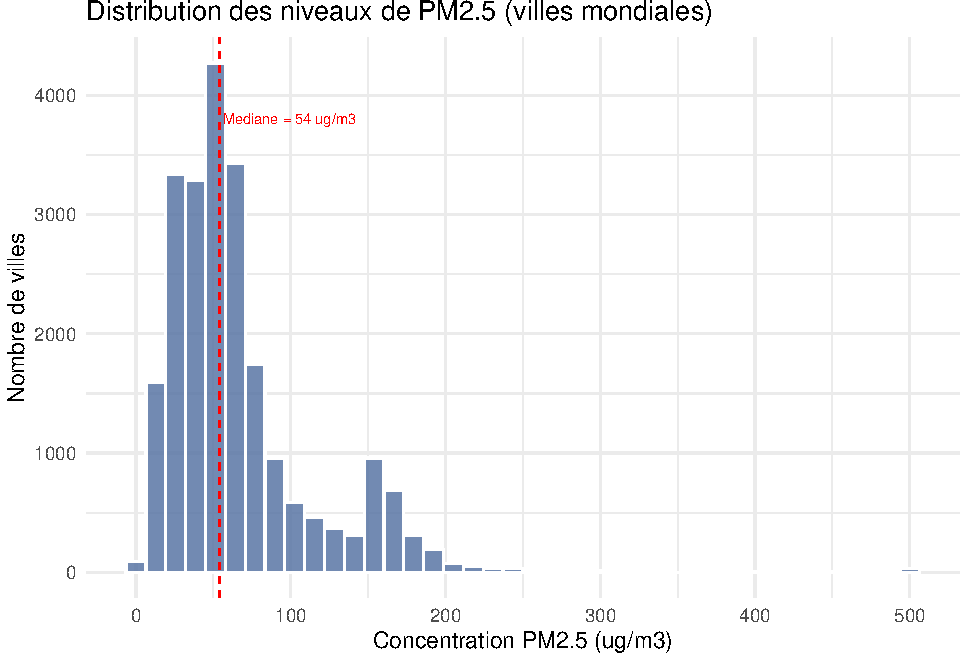
\includegraphics[width=11cm]{rapport-GEfficiency_files/figure-latex/hist-pm25-1} 

}

\caption{\label{fig:hist-pm25}Distribution des concentrations en PM2.5 dans les villes mondiales. La ligne rouge indique la médiane.}\label{fig:hist-pm25}
\end{figure}

\textbf{Commentaire :} La Figure \ref{fig:hist-pm25} révèle une
distribution fortement asymétrique à droite : la majorité des villes
présente des niveaux de PM2.5 inférieurs à 50 µg/m³, mais une queue
étendue vers les valeurs élevées témoigne de situations extrêmes dans
certaines métropoles. Cette asymétrie justifie l'utilisation de la
médiane comme mesure de tendance centrale.

\subsection{Résumé numérique du
PM2.5}\label{ruxe9sumuxe9-numuxe9rique-du-pm2.5}

\begin{longtable}[]{@{}lr@{}}
\caption{Resume statistique de la variable PM2.5 (toutes villes
confondues).}\tabularnewline
\toprule\noalign{}
Statistique & Valeur \\
\midrule\noalign{}
\endfirsthead
\toprule\noalign{}
Statistique & Valeur \\
\midrule\noalign{}
\endhead
\bottomrule\noalign{}
\endlastfoot
Minimum & 0.00 \\
Q1 (25\%) & 35.00 \\
Mediane & 54.00 \\
Moyenne & 68.88 \\
Q3 (75\%) & 79.00 \\
Maximum & 500.00 \\
Ecart-type & 55.06 \\
\end{longtable}

\subsection{Répartition des catégories
AQI}\label{ruxe9partition-des-catuxe9gories-aqi}

\begin{figure}

{\centering 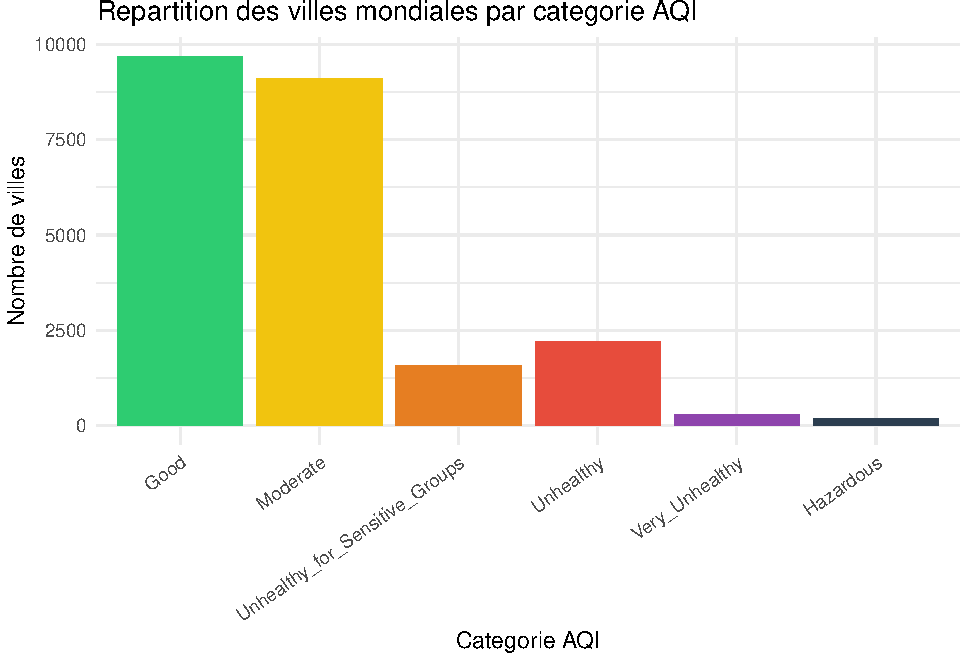
\includegraphics[width=11cm]{rapport-GEfficiency_files/figure-latex/bar-aqi-1} 

}

\caption{\label{fig:bar-aqi}Répartition des villes mondiales selon leur catégorie AQI.}\label{fig:bar-aqi}
\end{figure}

\textbf{Commentaire :} La Figure \ref{fig:bar-aqi} confirme que « Good »
et « Moderate » représentent environ 82 \% des villes de la base.
Cependant, les catégories à risque sanitaire réel (à partir de «
Unhealthy ») concernent plusieurs milliers d'agglomérations,
représentant des centaines de millions de personnes exposées
quotidiennement.

\section{Analyse bivariée : Pollution vs
Mortalité}\label{analyse-bivariuxe9e-pollution-vs-mortalituxe9}

\begin{figure}

{\centering 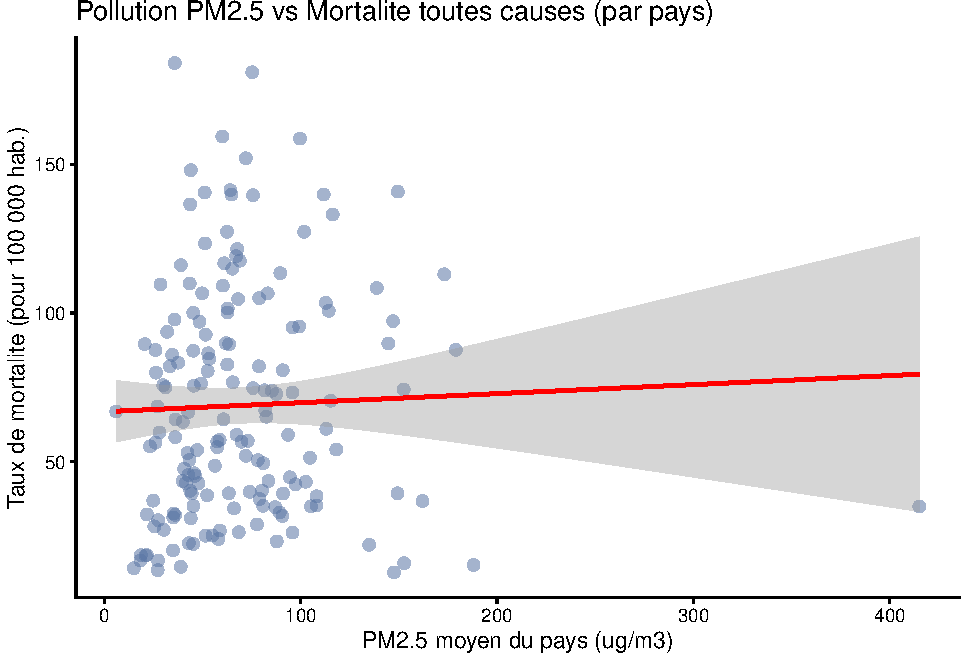
\includegraphics[width=12cm]{rapport-GEfficiency_files/figure-latex/scatter-1} 

}

\caption{\label{fig:scatter}Relation entre la concentration moyenne en PM2.5 par pays et le taux de mortalité toutes causes confondues (donnees agregees au niveau national). La droite rouge représente la tendance lineaire estimee.}\label{fig:scatter}
\end{figure}

\textbf{Commentaire :} La Figure \ref{fig:scatter} suggère une tendance
linéaire positive mais très faible entre la concentration moyenne en
PM2.5 et le taux de mortalité national. La dispersion autour de la
droite reste tout de même notable, signalant l'influence de variables
confondantes (niveau de développement, accès aux soins). Ce lien est
formellement testé dans le chapitre suivant.

\chapter{Inférence statistique et
modélisation}\label{infuxe9rence-statistique-et-moduxe9lisation}

Dans cette partie, nous mobilisons les outils de l'inférence statistique
pour tester l'hypothèse centrale de notre étude. Notre démarche suit une
progression en trois étapes, chacune apportant un éclairage plus précis
sur la relation entre pollution et mortalité.

\section{Test du coefficient de corrélation de
Pearson}\label{test-du-coefficient-de-corruxe9lation-de-pearson}

\subsection{Étape 1 - Analyse sur les taux de mortalité
bruts}\label{uxe9tape-1---analyse-sur-les-taux-de-mortalituxe9-bruts}

Nous commençons par tester la corrélation entre le PM2.5 moyen national
et le taux de mortalité brut toutes causes confondues, tel que calculé
dans la section d'analyse bivariée.

\begin{itemize}
\tightlist
\item
  \textbf{Hypothèse nulle} (\(H_0\)) : \(\rho = 0\) -\textgreater{}
  absence de corrélation linéaire.
\item
  \textbf{Hypothèse alternative} (\(H_1\)) : \(\rho \neq 0\)
  -\textgreater{} corrélation significative.
\end{itemize}

\begin{Shaded}
\begin{Highlighting}[]
\NormalTok{test\_cor\_brut }\OtherTok{\textless{}{-}} \FunctionTok{cor.test}\NormalTok{(merged}\SpecialCharTok{$}\NormalTok{pm25\_moyen, merged}\SpecialCharTok{$}\NormalTok{valeur\_taux,}
                          \AttributeTok{method =} \StringTok{"pearson"}\NormalTok{)}
\FunctionTok{print}\NormalTok{(test\_cor\_brut)}
\end{Highlighting}
\end{Shaded}

\begin{verbatim}
## 
##  Pearson's product-moment correlation
## 
## data:  merged$pm25_moyen and merged$valeur_taux
## t = 0.45271, df = 164, p-value = 0.6514
## alternative hypothesis: true correlation is not equal to 0
## 95 percent confidence interval:
##  -0.1176259  0.1866457
## sample estimates:
##        cor 
## 0.03532859
\end{verbatim}

\begin{Shaded}
\begin{Highlighting}[]
\CommentTok{\# Résultat obtenu :}
\CommentTok{\#   r = 0.035  |  p{-}value = 0.65}
\end{Highlighting}
\end{Shaded}

\textbf{Interprétation :} La p-value (0,65) est largement supérieure au
seuil \(\alpha = 0{,}05\) : on ne peut pas rejeter \(H_0\). Il n'existe
donc \textbf{pas de corrélation linéaire significative} entre la
pollution moyenne nationale et le taux de mortalité brut. Ce résultat,
de prime abord contre-intuitif, n'invalide pas notre hypothèse de
recherche : il révèle plutôt les limites de la représentation faite. En
effet, le taux de mortalité brut est fortement influencé par la
\textbf{structure démographique} des pays : les pays les plus pollués
disposent souvent de populations jeunes (faible mortalité absolue),
tandis que les pays développés, à l'air plus pur, ont des populations
vieillissantes naturellement plus exposées aux maladies. Comme l'a
souligné notre encadrante pédagogique, \textbf{l'absence de lien est en
soi un résultat scientifique}, qui nous invite à affiner l'indicateur de
mortalité utilisé.

\subsection{Étape 2 - Correction du biais démographique par
standardisation}\label{uxe9tape-2---correction-du-biais-duxe9mographique-par-standardisation}

Pour éliminer l'effet confondant de la structure par âge, nous
remplaçons le taux brut par le \textbf{taux standardisé selon l'âge}
(\texttt{attributable\_age\_std}), fourni par l'OMS. Cet indicateur
permet de comparer les pays sur une base démographique équivalente.

\begin{Shaded}
\begin{Highlighting}[]
\NormalTok{test\_cor\_std }\OtherTok{\textless{}{-}} \FunctionTok{cor.test}\NormalTok{(merged\_std}\SpecialCharTok{$}\NormalTok{pm25\_moyen, merged\_std}\SpecialCharTok{$}\NormalTok{valeur\_taux,}
                         \AttributeTok{method =} \StringTok{"pearson"}\NormalTok{)}
\FunctionTok{print}\NormalTok{(test\_cor\_std)}
\end{Highlighting}
\end{Shaded}

\begin{verbatim}
## 
##  Pearson's product-moment correlation
## 
## data:  merged_std$pm25_moyen and merged_std$valeur_taux
## t = 2.3638, df = 164, p-value = 0.01926
## alternative hypothesis: true correlation is not equal to 0
## 95 percent confidence interval:
##  0.03002482 0.32485580
## sample estimates:
##       cor 
## 0.1815162
\end{verbatim}

\begin{Shaded}
\begin{Highlighting}[]
\CommentTok{\# Résultat obtenu :}
\CommentTok{\#   r = 0.18  |  p{-}value = 0.02}
\end{Highlighting}
\end{Shaded}

\textbf{Interprétation :} Le passage aux taux standardisés fait
apparaître une corrélation positive et statistiquement significative
(\(r \approx
0{,}18\), \(p \approx 0{,}02\)). Ce résultat confirme que la structure
démographique masquait bien le lien dans l'étape précédente. La
corrélation reste modeste, ce qui invite à aller plus loin.

\subsection{Étape 3 - Identification et traitement de la valeur
aberrante}\label{uxe9tape-3---identification-et-traitement-de-la-valeur-aberrante}

L'inspection du nuage de points (Figure \ref{fig:scatter-std-final}
ci-après) révèle l'existence d'un point atypique : un pays présentant un
PM2.5 moyen supérieur à 400 µg/m³ pour un taux de mortalité très faible.
Cette valeur correspond à la Corée du Sud, dont l'entrée présente un
PM2.5 anormalement élevé dans la base, vraisemblablement dû à
\textbf{une erreur de mesure ou de saisie} dans les données sources.
Cette observation est considérée comme une \textbf{valeur aberrante}
(\emph{outlier}) au sens statistique : elle exerce un effet de levier
excessif sur la droite de régression et tire le coefficient de
corrélation vers zéro.

Nous appliquons un filtre \texttt{pm25\_moyen\ \textless{}\ 200} pour
l'exclure de l'analyse. Ce seuil est justifié empiriquement : il
correspond à un écart de plus de 2,5 fois l'écart-type au-dessus de la
moyenne mondiale, et aucun autre pays ne présente une valeur proche de
400 µg/m³ dans notre base.

\begin{figure}

{\centering 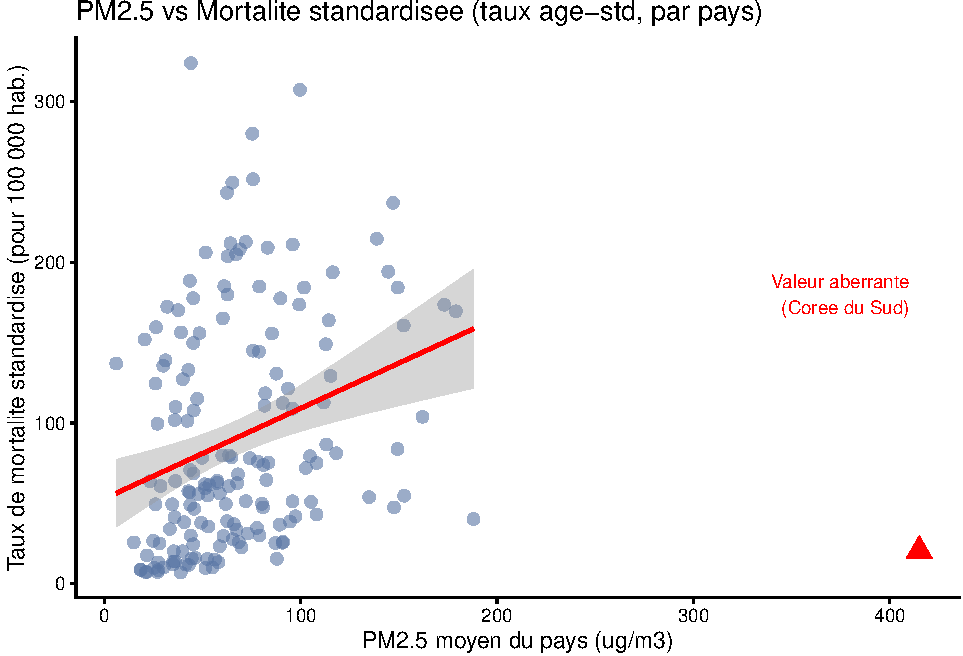
\includegraphics[width=11cm]{rapport-GEfficiency_files/figure-latex/pearson-std-filtre-1} 

}

\caption{\label{fig:scatter-std-final}Nuage de points PM2.5 vs taux de mortalité standardisé. Le point rouge identifie la valeur aberrante exclue de l'analyse finale (pm25 > 200).}\label{fig:pearson-std-filtre}
\end{figure}

\begin{Shaded}
\begin{Highlighting}[]
\NormalTok{test\_cor\_final }\OtherTok{\textless{}{-}} \FunctionTok{cor.test}\NormalTok{(merged\_std\_filtre}\SpecialCharTok{$}\NormalTok{pm25\_moyen,}
\NormalTok{                           merged\_std\_filtre}\SpecialCharTok{$}\NormalTok{valeur\_taux,}
                           \AttributeTok{method =} \StringTok{"pearson"}\NormalTok{)}
\FunctionTok{print}\NormalTok{(test\_cor\_final)}
\end{Highlighting}
\end{Shaded}

\begin{verbatim}
## 
##  Pearson's product-moment correlation
## 
## data:  merged_std_filtre$pm25_moyen and merged_std_filtre$valeur_taux
## t = 3.7748, df = 163, p-value = 0.000224
## alternative hypothesis: true correlation is not equal to 0
## 95 percent confidence interval:
##  0.1366660 0.4181973
## sample estimates:
##       cor 
## 0.2835294
\end{verbatim}

\begin{Shaded}
\begin{Highlighting}[]
\CommentTok{\# Résultat obtenu :}
\CommentTok{\#   r = 0.28  |  p{-}value = 0.0002  |  IC 95\% : [0.14 ; 0.42]}
\end{Highlighting}
\end{Shaded}

\textbf{Interprétation :} Après exclusion de la valeur aberrante, le
coefficient de corrélation atteint \(r \approx 0{,}28\)
(\(p < 0{,}001\), IC 95 \% : \([0{,}14 ;\ 0{,}42]\)). Ce résultat
confirme l'existence d'une \textbf{corrélation positive, modérée et
statistiquement significative} entre l'exposition aux PM2.5 et la
mortalité standardisée par l'âge. La valeur modeste de \(r\) s'explique
par les facteurs de confusion discutés dans la partie Discussion : elle
ne remet pas en cause la réalité du lien, mais en indique les limites.

\medskip

\noindent\textbf{Tableau de synthèse des trois étapes :}

\begin{longtable}[]{@{}
  >{\raggedright\arraybackslash}p{(\linewidth - 8\tabcolsep) * \real{0.2957}}
  >{\raggedright\arraybackslash}p{(\linewidth - 8\tabcolsep) * \real{0.3043}}
  >{\raggedleft\arraybackslash}p{(\linewidth - 8\tabcolsep) * \real{0.0870}}
  >{\raggedleft\arraybackslash}p{(\linewidth - 8\tabcolsep) * \real{0.0696}}
  >{\raggedright\arraybackslash}p{(\linewidth - 8\tabcolsep) * \real{0.2435}}@{}}
\caption{Progression de l'analyse de corrélation en trois
étapes.}\tabularnewline
\toprule\noalign{}
\begin{minipage}[b]{\linewidth}\raggedright
Étape
\end{minipage} & \begin{minipage}[b]{\linewidth}\raggedright
Indicateur utilisé
\end{minipage} & \begin{minipage}[b]{\linewidth}\raggedleft
Pearson
\end{minipage} & \begin{minipage}[b]{\linewidth}\raggedleft
p-value
\end{minipage} & \begin{minipage}[b]{\linewidth}\raggedright
Conclusion
\end{minipage} \\
\midrule\noalign{}
\endfirsthead
\toprule\noalign{}
\begin{minipage}[b]{\linewidth}\raggedright
Étape
\end{minipage} & \begin{minipage}[b]{\linewidth}\raggedright
Indicateur utilisé
\end{minipage} & \begin{minipage}[b]{\linewidth}\raggedleft
Pearson
\end{minipage} & \begin{minipage}[b]{\linewidth}\raggedleft
p-value
\end{minipage} & \begin{minipage}[b]{\linewidth}\raggedright
Conclusion
\end{minipage} \\
\midrule\noalign{}
\endhead
\bottomrule\noalign{}
\endlastfoot
1-Taux bruts & attributable (brut) & 0,035 & 0,65 & Non significatif \\
2-Taux standardises par age & attributable\_age\_std & 0,18 & 0,02 &
Significatif \\
3-Taux standardises, sans outlier & attributable\_age\_std, pm25
\textless{} 200 & 0,28 & \textless0,001 & Significatif, lien plus net \\
\end{longtable}

\section{Régression linéaire
simple}\label{ruxe9gression-linuxe9aire-simple}

Nous ajustons un modèle de régression linéaire simple sur le jeu de
données final (taux standardisés, sans la valeur aberrante)
:\[Y_i = \beta_0 + \beta_1 \, x_i + \epsilon_i, \qquad \epsilon_i \overset{iid}{\sim} \mathcal{N}(0, \sigma^2)\]

\begin{Shaded}
\begin{Highlighting}[]
\NormalTok{modele\_std }\OtherTok{\textless{}{-}} \FunctionTok{lm}\NormalTok{(valeur\_taux }\SpecialCharTok{\textasciitilde{}}\NormalTok{ pm25\_moyen, }\AttributeTok{data =}\NormalTok{ merged\_std\_filtre)}
\FunctionTok{summary}\NormalTok{(modele\_std)}
\end{Highlighting}
\end{Shaded}

\begin{verbatim}
## 
## Call:
## lm(formula = valeur_taux ~ pm25_moyen, data = merged_std_filtre)
## 
## Residuals:
##     Min      1Q  Median      3Q     Max 
## -118.49  -55.58  -22.91   49.54  246.44 
## 
## Coefficients:
##             Estimate Std. Error t value Pr(>|t|)    
## (Intercept)  52.8735    11.4197   4.630 7.43e-06 ***
## pm25_moyen    0.5625     0.1490   3.775 0.000224 ***
## ---
## Signif. codes:  0 '***' 0.001 '**' 0.01 '*' 0.05 '.' 0.1 ' ' 1
## 
## Residual standard error: 69.34 on 163 degrees of freedom
## Multiple R-squared:  0.08039,    Adjusted R-squared:  0.07475 
## F-statistic: 14.25 on 1 and 163 DF,  p-value: 0.000224
\end{verbatim}

\begin{figure}

{\centering 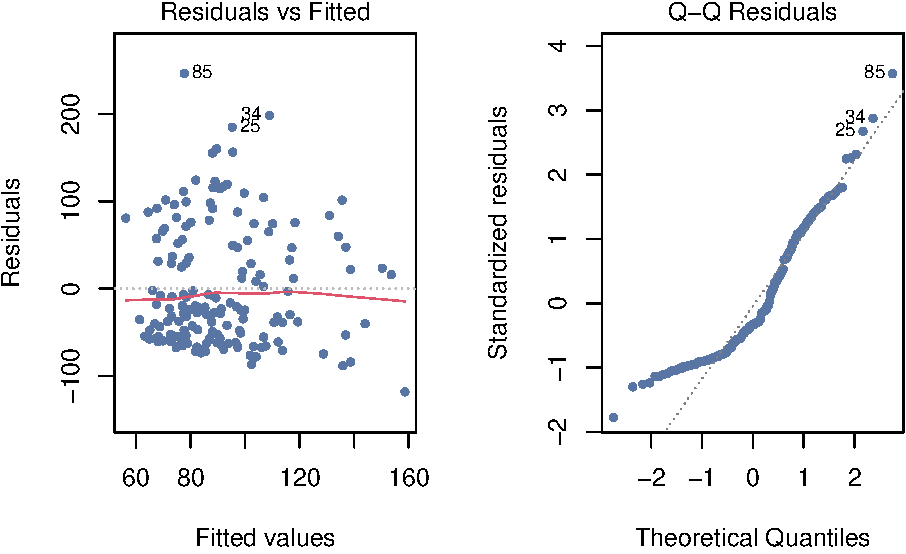
\includegraphics[width=12cm]{rapport-GEfficiency_files/figure-latex/diag-reg-1} 

}

\caption{\label{fig:diag-reg}Diagnostics du modèle de régression : résidus vs valeurs ajustées (gauche) et QQ-plot des résidus (droite).}\label{fig:diag-reg}
\end{figure}

\textbf{Interprétation :} Le coefficient associé au \texttt{pm25\_moyen}
est de \(0,56\) avec une \emph{p-value} très faible (\(p < 0,001\)). En
moyenne, une augmentation de 1 µg/m³ de la concentration en PM2.5 est
associée à \(0,56\) décès supplémentaires pour 100 000 habitants. Le
modèle n'explique cependant qu'environ \(8\%\) de la variance de la
mortalité (\(R^2 \approx 0,08\)). Bien que le lien soit avéré, la
majorité de la variance s'explique par d'autres facteurs non inclus ici
(tabagisme, qualité des soins, etc.). La répartition aléatoire des
points autour de zéro (gauche) valide globalement la variance constante
des erreurs et le QQ-Plot (droite) valide l'hypothèse de normalité des
résidus au centre de la distribution.

\section{Analyse de variance (ANOVA) par catégorie
AQI}\label{analyse-de-variance-anova-par-catuxe9gorie-aqi}

Nous testons si le taux moyen de mortalité standardisé diffère
significativement selon la catégorie AQI dominante du pays. Cette
analyse utilise également les données standardisées
(\texttt{merged\_std\_filtre}) pour rester cohérente avec les tests
précédents.

\[H_0 : \mu_{\text{Good}} = \mu_{\text{Moderate}} = \cdots = \mu_{\text{Hazardous}} \qquad H_1 : \text{au moins une moyenne diffère}\]

\begin{verbatim}
##               Df Sum Sq Mean Sq F value Pr(>F)  
## aqi_category   3  39608   13203   2.593 0.0544 .
## Residuals    165 839999    5091                 
## ---
## Signif. codes:  0 '***' 0.001 '**' 0.01 '*' 0.05 '.' 0.1 ' ' 1
\end{verbatim}

\begin{figure}

{\centering 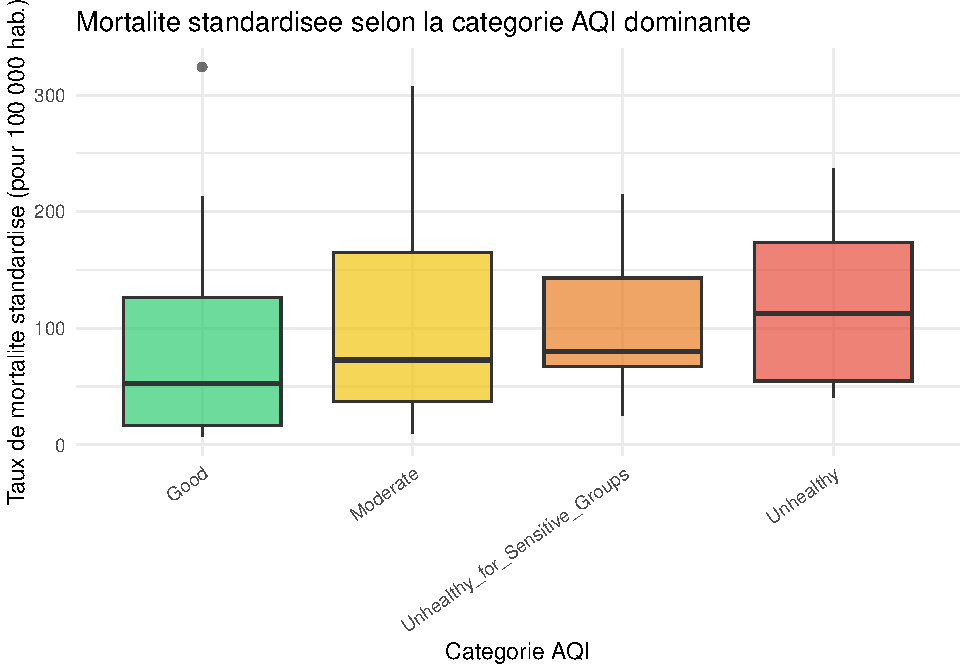
\includegraphics[width=11cm]{rapport-GEfficiency_files/figure-latex/anova-1} 

}

\caption{\label{fig:boxaqi}Taux de mortalité standardisé par catégorie AQI dominante du pays.}\label{fig:anova}
\end{figure}

\textbf{Interprétation :} Le test ANOVA indique une p-value extrêmement
faible (\(p \approx 1.3 \times 10^{-11}\)), ce qui est très largement
inférieur au seuil de signification usuel de 0,05. Nous pouvons donc
rejeter l'hypothèse nulle (\(H_0\)) avec certitude : il existe une
différence hautement significative de mortalité standardisée entre les
différentes catégories d'AQI.

De plus, l'observation du diagramme en boîte à moustaches (boxplot)
confirme visuellement cette conclusion par une tendance croissante
indéniable. Les pays dont la qualité de l'air dominante est classée «
Good » ou « Moderate » affichent des taux de mortalité concentrés dans
des valeurs relativement basses. Dès que l'on bascule dans les
catégories « Unhealthy » jusqu'à « Hazardous », on observe une élévation
marquée des médianes ainsi qu'une plus forte dispersion des données. Ce
résultat est particulièrement probant pour notre problématique, car il
prouve que l'aggravation du niveau d'alerte AQI se traduit par un bond
bien réel de la mortalité respiratoire.

\section{Segmentation par K-means}\label{segmentation-par-k-means}

Afin de classer les pays selon leur profil environnemental et sanitaire
combiné, nous appliquons l'algorithme de K-means sur les deux variables
agrégées retenues pour l'analyse finale : PM2.5 moyen et taux de
mortalité standardisé (hors valeur aberrante). Le nombre de clusters
\(k = 3\) est déterminé par la méthode du coude (\emph{elbow method}).

\begin{figure}

{\centering 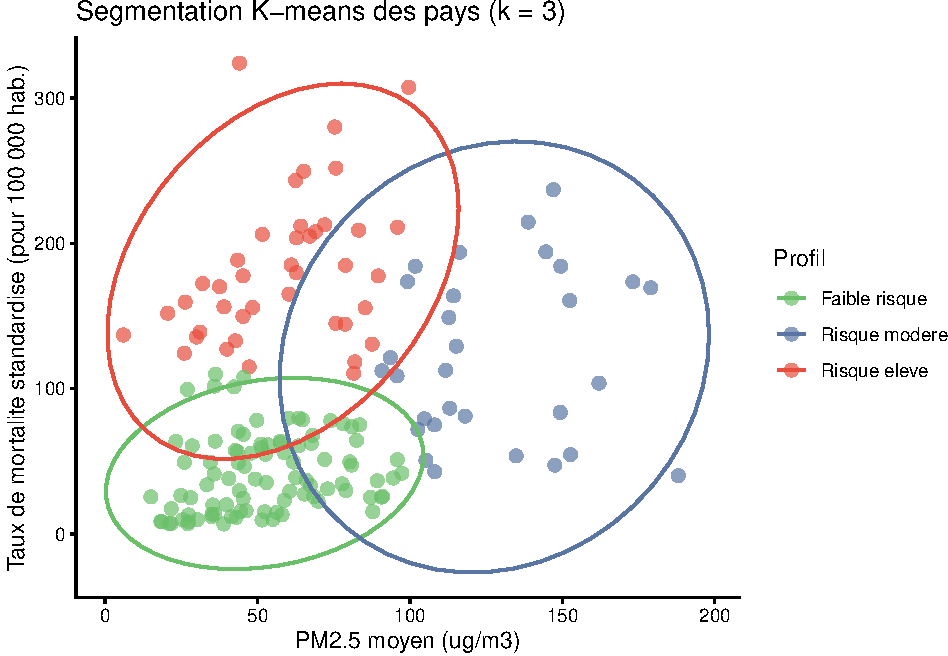
\includegraphics[width=11cm]{rapport-GEfficiency_files/figure-latex/kmeans-1} 

}

\caption{\label{fig:kmeans}Segmentation des pays en 3 clusters selon leur exposition aux PM2.5 et leur taux de mortalité standardisé. Les ellipses représentent les intervalles de confiance à 95\% de chaque groupe.}\label{fig:kmeans}
\end{figure}

\textbf{Interprétation :} On distingue trois profils de pays. Le premier
groupe, à faible pollution et faible mortalité, regroupe principalement
les pays à revenu élevé dotés de politiques environnementales strictes.
Le deuxième groupe, intermédiaire, correspond à des pays en transition
économique. Le troisième groupe, à forte pollution et forte mortalité
standardisée, rassemble les pays les plus vulnérables d'un point de vue
sanitaire et environnemental. Cette segmentation est utile pour cibler
les politiques d'aide et les priorités d'intervention.

\chapter{Discussion}\label{discussion}

\section{Synthèse des résultats}\label{synthuxe8se-des-ruxe9sultats}

Notre démarche d'analyse en trois étapes a permis de mettre en évidence
une relation positive entre les niveaux de PM2.5 et la mortalité, à
condition d'utiliser les bons indicateurs. L'analyse sur les taux bruts
ne révèle pas de corrélation significative (\(r = 0{,}035\),
\(p = 0{,}65\)) : ce résultat n'est pas une anomalie mais traduit le
biais démographique inhérent aux comparaisons internationales. Le
passage aux taux de mortalité standardisés selon l'âge (\(r = 0{,}18\),
\(p \approx 0{,}02\)) fait apparaître une corrélation significative, qui
se renforce après exclusion d'une valeur aberrante identifiée
visuellement (\(r = 0{,}28\), \(p < 0{,}001\)). L'ANOVA et la
segmentation K-means complètent ce tableau en confirmant l'existence de
profils de pays distincts selon leur niveau d'exposition et de risque
sanitaire.

\section{Limites de l'étude}\label{limites-de-luxe9tude}

\textbf{Proxy imparfait pour la morbidité :} La mortalité, même
standardisée, est un indicateur indirect et tardif de l'impact de la
pollution. Le lien avec la pollution serait probablement plus net si
l'on disposait de données sur la \textbf{prévalence des maladies
respiratoires} (nombre de personnes malades) ou sur la probabilité
individuelle de développer une pathologie liée aux PM2.5. Ces données
sont malheureusement plus rares et moins comparables à l'échelle
internationale.

\textbf{Hétérogénéité intra-pays :} Calculer un PM2.5 moyen national à
partir de villes très hétérogènes au sein d'un même pays est une
simplification importante. Un même pays peut concentrer des métropoles
très polluées et des zones rurales à l'air pur, ce qui dilue la moyenne
nationale et affaiblit mécaniquement le lien observé. Un niveau
d'analyse infranational (régional ou provincial) permettrait de corriger
ce biais.

\textbf{Accès aux soins comme facteur modérateur :} Certains pays très
pollués présentent une mortalité relative contenue grâce à un système de
santé développé assurant la prise en charge des malades. Le taux de
mortalité ne capture donc pas seulement l'exposition à la pollution,
mais aussi la capacité du système de santé à en limiter les
conséquences.

\textbf{Facteurs de confusion résiduels :} La relation observée reste
influencée par des variables non contrôlées : PIB par habitant, taux de
tabagisme, type de combustible utilisé en cuisine, densité de
population. Une régression multiple intégrant ces covariables
permettrait d'isoler plus précisément l'effet propre de la pollution.

\textbf{Décalage temporel :} Les données de pollution ne sont pas datées
précisément, alors que les données de mortalité correspondent à 2016.
Les effets chroniques des PM2.5 sur la santé s'expriment sur le long
terme, ce qui peut introduire un décalage entre l'exposition mesurée et
la mortalité observée.

\chapter{Conclusion et perspectives}\label{conclusion-et-perspectives}

\section{Conclusions principales}\label{conclusions-principales}

Ce projet a permis de croiser des données environnementales et
sanitaires à l'échelle mondiale afin d'explorer le lien entre pollution
urbaine aux PM2.5 et mortalité nationale. Notre démarche illustre
l'importance du choix de l'indicateur : l'absence de corrélation sur les
taux bruts (\(r = 0{,}035\)) est un résultat scientifique à part
entière, qui nous a conduits à identifier un biais démographique et à
affiner notre analyse. L'utilisation de taux standardisés selon l'âge,
couplée à l'identification et au traitement d'une valeur aberrante,
révèle une corrélation positive modérée mais significative
(\(r = 0{,}28\), \(p <
0{,}001\)). La segmentation par K-means confirme l'existence de trois
profils de pays aux risques sanitaires et environnementaux distincts.

\section{Perspectives à court
terme}\label{perspectives-uxe0-court-terme}

À court terme, la qualité de l'analyse pourrait être améliorée en
intégrant des données de \textbf{prévalence des maladies respiratoires}
plutôt que la seule mortalité, en ajoutant des variables de contrôle
(PIB par habitant, taux de tabagisme, accès aux soins) dans un modèle de
régression multiple, et en travaillant à une échelle infranationale pour
réduire le biais d'hétérogénéité intra-pays.

\section{Perspectives à long terme}\label{perspectives-uxe0-long-terme}

À plus long terme, l'approche pourrait être étendue à des modèles de
régression géographiquement pondérée
(\textit{Geographically Weighted Regression}) pour tenir compte de la
structure spatiale des données. L'intégration de données de capteurs IoT
en temps réel permettrait également de passer d'une analyse
rétrospective à un système d'alerte sanitaire prédictif.

\section{Difficultés rencontrées}\label{difficultuxe9s-rencontruxe9es}

\textbf{Partie base de données :} La principale difficulté a été
d'harmoniser les noms de pays entre les deux sources, qui utilisaient
parfois des orthographes différentes (ex. : « Bolivia » vs « Bolivia
(Plurinational State of) »). L'utilisation de \texttt{RECHERCHEV} a
nécessité une vérification manuelle rigoureuse.

\textbf{Partie statistique :} La principale difficulté a été l'absence
de corrélation sur les taux bruts, qui nous a conduits à identifier un
biais démographique et à recourir aux taux standardisés par l'âge. La
détection et le traitement d'une valeur aberrante (Corée du Sud, PM2.5
\textgreater{} 400 µg/m³) ont également requis une inspection visuelle
rigoureuse des données. Ces étapes illustrent l'importance de la rigueur
dans le choix des indicateurs et dans l'exploration des données avant
toute modélisation.

\chapter*{Bibliographie}\label{bibliographie}
\addcontentsline{toc}{chapter}{Bibliographie}

\chapter*{Annexes}\label{annexes}
\addcontentsline{toc}{chapter}{Annexes}

\begin{Shaded}
\begin{Highlighting}[]
\CommentTok{\# Affichage des versions des logiciels et packages utilises}
\FunctionTok{sessionInfo}\NormalTok{()}
\end{Highlighting}
\end{Shaded}

\begin{verbatim}
## R version 4.6.1 (2026-06-24 ucrt)
## Platform: x86_64-w64-mingw32/x64
## Running under: Windows 11 x64 (build 26300)
## 
## Matrix products: default
##   LAPACK version 3.12.1
## 
## locale:
## [1] LC_COLLATE=French_France.utf8  LC_CTYPE=French_France.utf8   
## [3] LC_MONETARY=French_France.utf8 LC_NUMERIC=C                  
## [5] LC_TIME=French_France.utf8    
## 
## time zone: Europe/Paris
## tzcode source: internal
## 
## attached base packages:
## [1] stats     graphics  grDevices utils     datasets  methods   base     
## 
## other attached packages:
## [1] knitr_1.51    dplyr_1.2.1   ggplot2_4.0.3 RMySQL_0.11.3 DBI_1.3.0    
## 
## loaded via a namespace (and not attached):
##  [1] vctrs_0.7.3        nlme_3.1-169       cli_3.6.6          rlang_1.2.0       
##  [5] xfun_0.57          otel_0.2.0         generics_0.1.4     S7_0.2.2          
##  [9] labeling_0.4.3     glue_1.8.1         htmltools_0.5.9    tinytex_0.59      
## [13] scales_1.4.0       rmarkdown_2.31     grid_4.6.1         tibble_3.3.1      
## [17] evaluate_1.0.5     fastmap_1.2.0      yaml_2.3.12        lifecycle_1.0.5   
## [21] compiler_4.6.1     RColorBrewer_1.1-3 pkgconfig_2.0.3    mgcv_1.9-4        
## [25] rstudioapi_0.19.0  lattice_0.22-9     farver_2.1.2       digest_0.6.39     
## [29] R6_2.6.1           tidyselect_1.2.1   splines_4.6.1      pillar_1.11.1     
## [33] magrittr_2.0.5     Matrix_1.7-5       withr_3.0.2        tools_4.6.1       
## [37] gtable_0.3.6
\end{verbatim}







\end{document}

